\documentclass[tikz,border=3pt]{standalone}
\usepackage[utf8]{inputenc}
\usepackage[T1]{fontenc}
\usepackage{lmodern}
\renewcommand{\familydefault}{\sfdefault}
\usepackage{sansmath}\sansmath
\usepackage{chemfig}
\usepackage{pgfplots}\pgfplotsset{compat=1.18,/pgf/number format/use comma,/pgf/number format/1000 sep={.}}
\usetikzlibrary{arrows.meta,calc,positioning,decorations.pathmorphing,patterns}
% paleta del sitio
\definecolor{nar}{HTML}{E8680C}\definecolor{narc}{HTML}{FFB35C}\definecolor{hielo}{HTML}{FFF3E8}
\definecolor{tinta}{HTML}{1D1D1F}\definecolor{gris}{HTML}{6E6E73}\definecolor{lila}{HTML}{7C5CF0}
\definecolor{azul}{HTML}{2F6FD6}\definecolor{menta}{HTML}{17A673}\definecolor{coral}{HTML}{E8342A}
\begin{document}
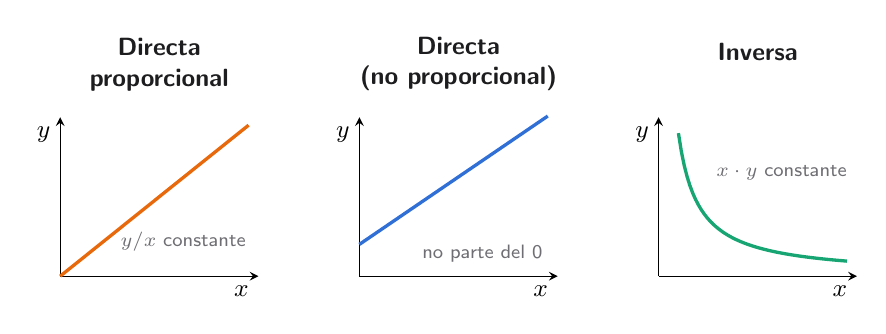
\begin{tikzpicture}[font=\small]
\pgfplotsset{mini/.style={width=4.1cm,height=3.6cm,axis lines=left,xtick=\empty,ytick=\empty,xmin=0,xmax=10,ymin=0,ymax=10,
  xlabel={$x$},ylabel={$y$},xlabel style={at={(axis description cs:1,0)},anchor=north east},ylabel style={rotate=-90,at={(axis description cs:0,1)},anchor=north east},
  title style={font=\small\bfseries,text=tinta,align=center},clip=false}}
\begin{axis}[mini,title={Directa\\proporcional},at={(0,0)}]
\addplot[nar,very thick,domain=0:9.5] {x};
\node[font=\scriptsize,text=gris] at (axis cs:6.2,2.2) {$y/x$ constante};
\end{axis}
\begin{axis}[mini,title={Directa\\(no proporcional)},at={(3.8cm,0)}]
\addplot[azul,very thick,domain=0:9.5] {2+0.85*x};
\node[font=\scriptsize,text=gris] at (axis cs:6.2,1.4) {no parte del 0};
\end{axis}
\begin{axis}[mini,title={Inversa\\\phantom{x}},at={(7.6cm,0)}]
\addplot[menta,very thick,domain=1:9.5,samples=60] {9/x};
\node[font=\scriptsize,text=gris] at (axis cs:6.2,6.5) {$x\cdot y$ constante};
\end{axis}
\end{tikzpicture}
\end{document}
